% =====================================================================
% AI Academy -- National AI Center
% Software Engineering Final Project -- Team Presentation Deck
% Topic 4 -- Async Research Assistant
%
% Built from templates/SLIDES_TEMPLATE.tex. Compile with pdfLaTeX.
% A PowerPoint rendering of the same slides is slides.pptx.
% Filled in for team-M503-SWE-06. No TODO markers remain.
% =====================================================================

\PassOptionsToPackage{dvipsnames}{xcolor}
\documentclass[aspectratio=169,11pt]{beamer}

% ===== EARLY MACROS ==================================================
\definecolor{accent2}{HTML}{8B0000}
\newcommand{\TODO}[1]{\textcolor{accent2}{\textbf{[TODO: #1]}}}

% ===== CONFIGURATION =================================================
\newcommand{\teamname}{team-M503-SWE-06}
\newcommand{\topicchoice}{Topic 4 -- Async Research Assistant}
\newcommand{\memberone}{Sanan Garibli}
\newcommand{\membertwo}{Humbat Camalov}
\newcommand{\memberthree}{Farah Nematzada}
\newcommand{\repolink}{github.com/team-M503-SWE-06/research-assistant}

\newcommand{\coursecode}{AI-ENG-110}
\newcommand{\coursename}{Software Engineering}
\newcommand{\institution}{AI Academy, National AI Center}
\newcommand{\semester}{Spring 2026}

% ===== PACKAGES ======================================================
\usepackage[T1]{fontenc}
\usepackage[utf8]{inputenc}
\usepackage{xcolor}
\usepackage{tabularx}
\usepackage{booktabs}
\usepackage{listings}
\usepackage{tikz}
\usetikzlibrary{shapes.geometric,arrows.meta,positioning,fit,backgrounds}

% ===== BEAMER THEME ==================================================
\usetheme{default}
\usefonttheme{professionalfonts}
\setbeamertemplate{navigation symbols}{}

\definecolor{accent}{HTML}{0B3D91}
\definecolor{soft}{HTML}{F2F4F8}
\definecolor{ok}{HTML}{166534}

\setbeamercolor{title}{fg=accent}
\setbeamercolor{frametitle}{fg=accent}
\setbeamercolor{section in head/foot}{bg=accent,fg=white}
\setbeamercolor{itemize item}{fg=accent}
\setbeamercolor{itemize subitem}{fg=accent}
\setbeamercolor{enumerate item}{fg=accent}
\setbeamercolor{block title}{bg=accent,fg=white}
\setbeamercolor{block body}{bg=soft,fg=black}

\setbeamerfont{title}{size=\Large,series=\bfseries}
\setbeamerfont{frametitle}{size=\large,series=\bfseries}
\setbeamerfont{footline}{size=\tiny}

\setbeamertemplate{footline}{%
  \leavevmode%
  \hbox to\paperwidth{\hspace*{2ex}\tiny\textit{\teamname{} -- \topicchoice}\hfill%
  \tiny\textit{\coursecode{}}\hfill%
  \tiny\insertframenumber/\inserttotalframenumber\hspace*{2ex}}%
  \vskip1pt%
}

% ===== CODE LISTINGS =================================================
\definecolor{codegreen}{rgb}{0,0.55,0}
\definecolor{codepurple}{rgb}{0.55,0,0.78}
\lstdefinestyle{python}{
  language=Python,
  backgroundcolor=\color{soft},
  commentstyle=\color{codegreen},
  keywordstyle=\color{accent},
  stringstyle=\color{codepurple},
  basicstyle=\ttfamily\scriptsize,
  breaklines=true,
  frame=single,
  framerule=0.4pt,
  rulecolor=\color{black!30},
  showstringspaces=false,
}

% =====================================================================

\begin{document}

% ========== 1 TITLE ==================================================
{%
\setbeamertemplate{footline}{}
\begin{frame}[plain]
  \begin{center}
    \vspace{0.6cm}
    {\small \textsc{\institution}}\\[0.2em]
    {\small \textsc{\coursecode{} -- \coursename{}}}\\[1.2em]
    \rule{0.7\textwidth}{0.6pt}\\[0.4em]
    {\Huge\bfseries\color{accent} \topicchoice}\\[0.3em]
    {\normalsize Three sources, queried in parallel, answered with citations}\\[0.4em]
    \rule{0.7\textwidth}{0.6pt}\\[1.0em]
    {\large \teamname}\\[0.6em]
    {\normalsize \memberone\quad\textbullet\quad\membertwo\quad\textbullet\quad\memberthree}\\[0.9cm]
    {\footnotesize\itshape Final Project Defense -- September 2026}\\[0.4em]
    {\footnotesize\texttt{\repolink}}
  \end{center}
\end{frame}
}

% ========== 2 PROBLEM ================================================
\begin{frame}{The problem in one sentence}
  \begin{block}{What the system does}
    A user asks a research question from the command line; we query Wikipedia, arXiv and a
    web-search API \emph{concurrently}, bounded by a per-source timeout, and return one
    LLM-synthesised paragraph whose every claim carries a numbered citation --- even when one of the
    three sources is down.
  \end{block}

  \vspace{0.2em}
  \begin{columns}[T,onlytextwidth]
  \column{0.48\textwidth}
  \textbf{Inputs}
  \begin{itemize}\setlength\itemsep{1pt}
    \item Question string (trimmed, non-empty, $\le$\,500 chars)
    \item \texttt{-{}-sources wiki,arxiv,web} subset
    \item \texttt{-{}-no-cache} to bypass the source cache
  \end{itemize}

  \column{0.48\textwidth}
  \textbf{Outputs}
  \begin{itemize}\setlength\itemsep{1pt}
    \item \texttt{ResearchSession}: answer with citations + one \texttt{SourceOutcome} per source
    \item Numbered references with URLs, per-source timing line
    \item Exit 0 (possibly degraded, with a note) or 1 with \texttt{Error: ...}
  \end{itemize}
  \end{columns}

  \vspace{0.3em}
  {\footnotesize\textbf{3} sources in parallel \quad$\cdot$\quad \textbf{13} modules,
  $\sim$620 lines \quad$\cdot$\quad \textbf{90} offline tests \quad$\cdot$\quad
  \textbf{95\,\%} statement coverage}
\end{frame}

% ========== 3 ARCHITECTURE ===========================================
\begin{frame}{Architecture}
  \textbf{One rule drove everything:} exactly one module imports \texttt{ai.*}.

  \vspace{0.2em}
  \begin{center}
  \hyphenpenalty=10000\exhyphenpenalty=10000\relax
  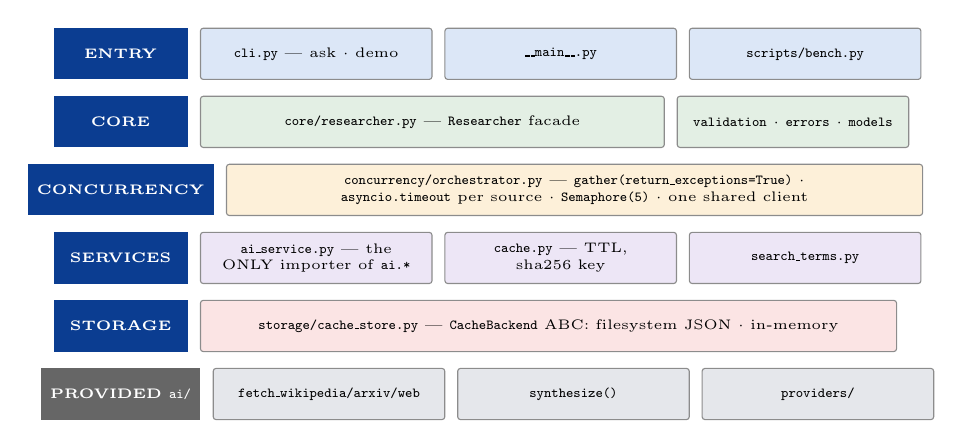
\begin{tikzpicture}[
    font=\tiny,
    band/.style={draw=black!45, rounded corners=1pt, minimum height=6.5mm, align=center, inner sep=2pt},
    lab/.style={draw=none, fill=accent, text=white, font=\tiny\bfseries,
                minimum height=6.5mm, minimum width=17mm, align=center},
  ]
  \definecolor{cEntry}{HTML}{DCE7F7}\definecolor{cCore}{HTML}{E3EFE4}
  \definecolor{cConc}{HTML}{FDF0D9}\definecolor{cServ}{HTML}{EDE6F6}
  \definecolor{cStor}{HTML}{FBE4E4}\definecolor{cProv}{HTML}{E5E7EB}

  \node[lab] (l1) {ENTRY};
  \node[band, fill=cEntry, right=1.5mm of l1, text width=28mm] (e1) {\texttt{cli.py} --- ask $\cdot$ demo};
  \node[band, fill=cEntry, right=1.5mm of e1, text width=28mm] (e2) {\texttt{\_\_main\_\_.py}};
  \node[band, fill=cEntry, right=1.5mm of e2, text width=28mm] (e3) {\texttt{scripts/bench.py}};

  \node[lab, below=2mm of l1] (l2) {CORE};
  \node[band, fill=cCore, right=1.5mm of l2, text width=57.5mm] (c1)
    {\texttt{core/researcher.py} --- \texttt{Researcher} facade};
  \node[band, fill=cCore, right=1.5mm of c1, text width=28mm] (c2) {\texttt{validation} $\cdot$ \texttt{errors} $\cdot$ \texttt{models}};

  \node[lab, below=2mm of l2] (l3) {CONCURRENCY};
  \node[band, fill=cConc, right=1.5mm of l3, text width=87mm] (o1)
    {\texttt{concurrency/orchestrator.py} --- \texttt{gather(return\_exceptions=True)} $\cdot$
     \texttt{asyncio.timeout} per source $\cdot$ \texttt{Semaphore(5)} $\cdot$ one shared client};

  \node[lab, below=2mm of l3] (l4) {SERVICES};
  \node[band, fill=cServ, right=1.5mm of l4, text width=28mm] (s1)
    {\texttt{ai\_service.py} --- the ONLY importer of \texttt{ai.*}};
  \node[band, fill=cServ, right=1.5mm of s1, text width=28mm] (s2) {\texttt{cache.py} --- TTL, sha256 key};
  \node[band, fill=cServ, right=1.5mm of s2, text width=28mm] (s3) {\texttt{search\_terms.py}};

  \node[lab, below=2mm of l4] (l5) {STORAGE};
  \node[band, fill=cStor, right=1.5mm of l5, text width=87mm] (st1)
    {\texttt{storage/cache\_store.py} --- \texttt{CacheBackend} ABC: filesystem JSON $\cdot$ in-memory};

  \node[lab, below=2mm of l5, fill=black!60] (l6) {PROVIDED \texttt{ai/}};
  \node[band, fill=cProv, right=1.5mm of l6, text width=28mm] (p1) {\texttt{fetch\_wikipedia/arxiv/web}};
  \node[band, fill=cProv, right=1.5mm of p1, text width=28mm] (p2) {\texttt{synthesize()}};
  \node[band, fill=cProv, right=1.5mm of p2, text width=28mm] (p3) {\texttt{providers/}};
  \end{tikzpicture}
  \end{center}

  \vspace{0.1em}
  {\footnotesize Dependencies point downward only. \texttt{bootstrap.build\_researcher()} is the
  single composition root --- the CLI and the benchmark get an identically wired object graph.}
\end{frame}

% ========== 4 DESIGN DECISIONS =======================================
\begin{frame}{Three design decisions we can defend}
  \begin{enumerate}\setlength\itemsep{6pt}
    \item \textbf{One choke point for \texttt{ai.*}.} \texttt{AIService} is the only module that
    imports the provided package. Makes ``never call provider SDKs from business logic'' checkable
    by grep, and gives retries, timeouts and logging exactly one home.

    \item \textbf{A \texttt{CacheBackend} ABC, composed --- not inherited --- into
    \texttt{SourceCache}.} Two implementations that share no code: one JSON file per key, or a dict
    for tests. TTL policy is orthogonal to storage, so composing avoids a class per
    (policy $\times$ storage) pair. Swapping in PostgreSQL is one subclass and one line in bootstrap.

    \item \textbf{A long-lived semaphore and HTTP client, owned by the orchestrator.} A per-call
    semaphore bounds nothing once several questions run at once. Building the SSL trust store costs
    $\sim$0.35\,s and was being paid per client --- hoisting it makes every later client nearly free.
  \end{enumerate}
\end{frame}

% ========== 5 CONCURRENCY + BENCHMARK ================================
\begin{frame}[fragile]{Concurrency: how it works, and what it buys}
  \begin{lstlisting}[style=python]
tasks = [self._run_one(o, question, use_cache, self._client) for o in requested]
results = await asyncio.gather(*tasks, return_exceptions=True)

async with self._semaphore:                              # global bound
    async with asyncio.timeout(per_source_timeout):      # per source
        sources = await fetch(question, ..., client=client)
  \end{lstlisting}

  \vspace{0.2em}
  {\footnotesize
  \textbf{\texttt{return\_exceptions=True}} --- one dead source does not cancel its siblings.\quad
  \textbf{timeout per task} --- a slow Wikipedia burns its own budget, not arXiv's.\quad
  \textbf{\texttt{Semaphore(5)}} --- bounds total in-flight calls, not per request.}

  \vspace{0.3em}
  \begin{center}\small
  \begin{tabular}{lccccc}
    \toprule
    \textbf{Workload} & \textbf{N} & \textbf{Sequential} & \textbf{Concurrent} & \textbf{Speedup} \\
    \midrule
    5 sample research questions & 5 & 31.4\,s & 8.8\,s & $\mathbf{3.6\times}$ \\
    \bottomrule
  \end{tabular}
  \end{center}

  \vspace{0.2em}
  {\footnotesize\itshape Captured 18 Sep 2026 $\cdot$ Windows 11, Intel 16-core, Python 3.13.14
  $\cdot$ \texttt{claude-sonnet-5} + Tavily $\cdot$ cache bypassed in both phases $\cdot$
  raw log committed at \texttt{artefacts/bench.md}.}
\end{frame}

% ========== 6 ROBUSTNESS =============================================
\begin{frame}{Robustness: one concrete failure mode}
  \textbf{Partial source failure --- the web search dies, the answer still ships.}

  \vspace{0.3em}
  \begin{itemize}\setlength\itemsep{4pt}
    \item \textbf{Injected.} A deliberately invalid Tavily key, no code changed. Also unit-tested by
    monkeypatching the arXiv fetcher to raise \texttt{ProviderError} on every attempt.
    \item \textbf{What happened.} \texttt{gather(return\_exceptions=True)} returned the exception
    instead of cancelling siblings; the orchestrator recorded
    \texttt{SourceOutcome(source\_count=0, error=...)}; the facade saw a non-empty source list and
    synthesised anyway.
    \item \textbf{What the user saw.} A complete cited answer, then one line:\\
    {\footnotesize\texttt{Note: web unavailable (Tavily search failed: Client error '401 Unauthorized')}}
    \item \textbf{The complement is tested too.} When \emph{every} source fails there is nothing
    honest to synthesise, so the facade raises \texttt{NoSourcesAvailableError} and the CLI exits 1
    with a one-line message --- never a traceback.
  \end{itemize}

  \vspace{0.2em}
  {\footnotesize Evidence: \texttt{artefacts/degraded-run.txt}, committed from a live run.}
\end{frame}

% ========== 7 DEMO ===================================================
\begin{frame}[fragile]{Demo}
  \begin{lstlisting}[style=python, language=bash]
$ python -m researcher ask "How does CRISPR-Cas9 gene editing work?"

A: CRISPR-Cas9 uses a guide RNA to direct the Cas9 nuclease to a matching
   DNA sequence, where it introduces a double-strand break [1][2]...

References:
  [1] (wikipedia) CRISPR gene editing
  [2] (arxiv)     Structural basis of Cas9 target recognition
  [3] (web)       How CRISPR works

(timing: wikipedia=0.37s, arxiv=0.38s, web=0.48s; * = cache hit)
  \end{lstlisting}

  \vspace{0.1em}
  \textbf{Fallbacks:} \texttt{-{}-sources wiki,arxiv} if the search key is rate-limited $\cdot$
  \texttt{demo} runs all five sample questions $\cdot$ a second run inside the TTL is served from
  cache and is visibly faster $\cdot$ \texttt{docker run -{}-env-file .env research-assistant}.
\end{frame}

% ========== 8 TESTING ================================================
\begin{frame}{Testing}
  \begin{center}\small
  \begin{tabular}{cccc}
    \toprule
    \textbf{90} & \textbf{95\,\%} & \textbf{16/16} & \textbf{60\,\%} \\
    tests, all offline & statement coverage & provided smoke tests & CI coverage gate \\
    \bottomrule
  \end{tabular}
  \end{center}

  \vspace{0.4em}
  \begin{itemize}\setlength\itemsep{4pt}
    \item \textbf{We mock at exactly one seam} --- the \texttt{ai.*} functions. Everything below is
    the real object graph: a real orchestrator, a real cache, a real retry policy. Mocking the
    orchestrator would have meant testing our mocks instead of our wiring.
    \item \textbf{The concurrency tests} pin what the design promises: one task raising does not
    cancel the others; a slow source trips its own timeout; the semaphore's observed peak never
    exceeds its bound; a cache hit is served \emph{before} a slot is taken.
    \item \textbf{The test that earned its keep:} printing an answer to a redirected stream on
    Windows raised \texttt{UnicodeEncodeError} mid-answer, after the user had already seen half of
    it. stdout is now reconfigured to UTF-8, and both that and the un-reconfigurable case are pinned.
  \end{itemize}
\end{frame}

% ========== 9 LIMITATIONS ============================================
\begin{frame}{Limitations \& what we would do next}
  \begin{itemize}\setlength\itemsep{4pt}
    \item \textbf{The search-term fallback is a heuristic, not a fix.} A stopword list and a sliding
    window tuned against five questions. A question whose topic word is also a stopword still does
    badly --- the real fix is an endpoint the contract will not let us call.
    \item \textbf{Cache keys ignore \texttt{max\_results}.} Ask for 3 then for 10 and you silently
    get 3. Not reachable from the CLI today, so it cannot bite yet --- but it is a latent bug.
    \item \textbf{The concurrency bound is global, not per-host.} A slow arXiv can hold slots
    Wikipedia could have used.
    \item \textbf{Nothing is persisted beyond the cache.} A \texttt{ResearchSession} is built,
    printed and dropped.
    \item \textbf{With another week:} per-host rate limiting $\rightarrow$ persist sessions
    $\rightarrow$ replace the keyword heuristic. In that order, because that is the order in which a
    user notices.
  \end{itemize}
\end{frame}

% ========== 10 CONTRIBUTIONS =========================================
\begin{frame}{Team contributions}
  \begin{center}\scriptsize
  \begin{tabularx}{\textwidth}{@{}lXc@{}}
    \toprule
    \textbf{Member} & \textbf{Pull requests} & \textbf{Share} \\
    \midrule
    Sanan Garibli & \#1 config \& models $\cdot$ \#4 orchestrator $\cdot$ \#7 tests $\cdot$ \#10 Docker \& CI $\cdot$ \#17 final & 5/17 \\
    \addlinespace
    Humbat Camalov & \#3 AIService $\cdot$ \#5 CLI \& benchmark $\cdot$ \#9 tests $\cdot$ \#12 artefacts $\cdot$ \#14 pitfall fixes $\cdot$ \#16 slides & 6/17 \\
    \addlinespace
    Farah Nematzada & \#2 cache \& storage $\cdot$ \#6 tests $\cdot$ \#8 tests $\cdot$ \#11 README $\cdot$ \#13 benchmark $\cdot$ \#15 report & 6/17 \\
    \bottomrule
  \end{tabularx}
  \end{center}

  \vspace{0.5em}
  \textbf{How we worked}
  \begin{itemize}\setlength\itemsep{2pt}
    \item Feature branches named \texttt{<member>/<short-description>}; \texttt{main} is protected.
    \item Every PR used the template: what changed, why, how it was tested, what it does \emph{not} do.
    \item The reviewer approves; the author merges. CI --- ruff, mypy, pytest with the coverage gate,
    and a Docker build --- must be green first.
  \end{itemize}
\end{frame}

% ========== 11 CLOSING ===============================================
{%
\setbeamertemplate{footline}{}
\begin{frame}[plain]
  \begin{center}
    \vspace{1.6cm}
    {\Huge\bfseries\color{accent} Thank you}\\[0.6em]
    {\large Questions?}\\[1.4cm]
    {\footnotesize\texttt{\repolink}}\\[0.4em]
    {\footnotesize \memberone\quad\textbullet\quad\membertwo\quad\textbullet\quad\memberthree}
  \end{center}
\end{frame}
}

\end{document}
